% Options for packages loaded elsewhere
\PassOptionsToPackage{unicode}{hyperref}
\PassOptionsToPackage{hyphens}{url}
\PassOptionsToPackage{dvipsnames,svgnames,x11names}{xcolor}
%
\documentclass[
  11pt,
  oneside]{book}
\usepackage{amsmath,amssymb}
\usepackage{lmodern}
\usepackage{iftex}
\ifPDFTeX
  \usepackage[T1]{fontenc}
  \usepackage[utf8]{inputenc}
  \usepackage{textcomp} % provide euro and other symbols
\else % if luatex or xetex
  \usepackage{unicode-math}
  \defaultfontfeatures{Scale=MatchLowercase}
  \defaultfontfeatures[\rmfamily]{Ligatures=TeX,Scale=1}
\fi
% Use upquote if available, for straight quotes in verbatim environments
\IfFileExists{upquote.sty}{\usepackage{upquote}}{}
\IfFileExists{microtype.sty}{% use microtype if available
  \usepackage[]{microtype}
  \UseMicrotypeSet[protrusion]{basicmath} % disable protrusion for tt fonts
}{}
\makeatletter
\@ifundefined{KOMAClassName}{% if non-KOMA class
  \IfFileExists{parskip.sty}{%
    \usepackage{parskip}
  }{% else
    \setlength{\parindent}{0pt}
    \setlength{\parskip}{6pt plus 2pt minus 1pt}}
}{% if KOMA class
  \KOMAoptions{parskip=half}}
\makeatother
\usepackage{xcolor}
\usepackage[left=1in,right=1in,top=1.5in,bottom=1.5in]{geometry}
\usepackage{color}
\usepackage{fancyvrb}
\newcommand{\VerbBar}{|}
\newcommand{\VERB}{\Verb[commandchars=\\\{\}]}
\DefineVerbatimEnvironment{Highlighting}{Verbatim}{commandchars=\\\{\}}
% Add ',fontsize=\small' for more characters per line
\usepackage{framed}
\definecolor{shadecolor}{RGB}{248,248,248}
\newenvironment{Shaded}{\begin{snugshade}}{\end{snugshade}}
\newcommand{\AlertTok}[1]{\textcolor[rgb]{0.94,0.16,0.16}{#1}}
\newcommand{\AnnotationTok}[1]{\textcolor[rgb]{0.56,0.35,0.01}{\textbf{\textit{#1}}}}
\newcommand{\AttributeTok}[1]{\textcolor[rgb]{0.77,0.63,0.00}{#1}}
\newcommand{\BaseNTok}[1]{\textcolor[rgb]{0.00,0.00,0.81}{#1}}
\newcommand{\BuiltInTok}[1]{#1}
\newcommand{\CharTok}[1]{\textcolor[rgb]{0.31,0.60,0.02}{#1}}
\newcommand{\CommentTok}[1]{\textcolor[rgb]{0.56,0.35,0.01}{\textit{#1}}}
\newcommand{\CommentVarTok}[1]{\textcolor[rgb]{0.56,0.35,0.01}{\textbf{\textit{#1}}}}
\newcommand{\ConstantTok}[1]{\textcolor[rgb]{0.00,0.00,0.00}{#1}}
\newcommand{\ControlFlowTok}[1]{\textcolor[rgb]{0.13,0.29,0.53}{\textbf{#1}}}
\newcommand{\DataTypeTok}[1]{\textcolor[rgb]{0.13,0.29,0.53}{#1}}
\newcommand{\DecValTok}[1]{\textcolor[rgb]{0.00,0.00,0.81}{#1}}
\newcommand{\DocumentationTok}[1]{\textcolor[rgb]{0.56,0.35,0.01}{\textbf{\textit{#1}}}}
\newcommand{\ErrorTok}[1]{\textcolor[rgb]{0.64,0.00,0.00}{\textbf{#1}}}
\newcommand{\ExtensionTok}[1]{#1}
\newcommand{\FloatTok}[1]{\textcolor[rgb]{0.00,0.00,0.81}{#1}}
\newcommand{\FunctionTok}[1]{\textcolor[rgb]{0.00,0.00,0.00}{#1}}
\newcommand{\ImportTok}[1]{#1}
\newcommand{\InformationTok}[1]{\textcolor[rgb]{0.56,0.35,0.01}{\textbf{\textit{#1}}}}
\newcommand{\KeywordTok}[1]{\textcolor[rgb]{0.13,0.29,0.53}{\textbf{#1}}}
\newcommand{\NormalTok}[1]{#1}
\newcommand{\OperatorTok}[1]{\textcolor[rgb]{0.81,0.36,0.00}{\textbf{#1}}}
\newcommand{\OtherTok}[1]{\textcolor[rgb]{0.56,0.35,0.01}{#1}}
\newcommand{\PreprocessorTok}[1]{\textcolor[rgb]{0.56,0.35,0.01}{\textit{#1}}}
\newcommand{\RegionMarkerTok}[1]{#1}
\newcommand{\SpecialCharTok}[1]{\textcolor[rgb]{0.00,0.00,0.00}{#1}}
\newcommand{\SpecialStringTok}[1]{\textcolor[rgb]{0.31,0.60,0.02}{#1}}
\newcommand{\StringTok}[1]{\textcolor[rgb]{0.31,0.60,0.02}{#1}}
\newcommand{\VariableTok}[1]{\textcolor[rgb]{0.00,0.00,0.00}{#1}}
\newcommand{\VerbatimStringTok}[1]{\textcolor[rgb]{0.31,0.60,0.02}{#1}}
\newcommand{\WarningTok}[1]{\textcolor[rgb]{0.56,0.35,0.01}{\textbf{\textit{#1}}}}
\usepackage{longtable,booktabs,array}
\usepackage{calc} % for calculating minipage widths
% Correct order of tables after \paragraph or \subparagraph
\usepackage{etoolbox}
\makeatletter
\patchcmd\longtable{\par}{\if@noskipsec\mbox{}\fi\par}{}{}
\makeatother
% Allow footnotes in longtable head/foot
\IfFileExists{footnotehyper.sty}{\usepackage{footnotehyper}}{\usepackage{footnote}}
\makesavenoteenv{longtable}
\usepackage{graphicx}
\makeatletter
\def\maxwidth{\ifdim\Gin@nat@width>\linewidth\linewidth\else\Gin@nat@width\fi}
\def\maxheight{\ifdim\Gin@nat@height>\textheight\textheight\else\Gin@nat@height\fi}
\makeatother
% Scale images if necessary, so that they will not overflow the page
% margins by default, and it is still possible to overwrite the defaults
% using explicit options in \includegraphics[width, height, ...]{}
\setkeys{Gin}{width=\maxwidth,height=\maxheight,keepaspectratio}
% Set default figure placement to htbp
\makeatletter
\def\fps@figure{htbp}
\makeatother
\setlength{\emergencystretch}{3em} % prevent overfull lines
\providecommand{\tightlist}{%
  \setlength{\itemsep}{0pt}\setlength{\parskip}{0pt}}
\setcounter{secnumdepth}{5}
\newlength{\cslhangindent}
\setlength{\cslhangindent}{1.5em}
\newlength{\csllabelwidth}
\setlength{\csllabelwidth}{3em}
\newlength{\cslentryspacingunit} % times entry-spacing
\setlength{\cslentryspacingunit}{\parskip}
\newenvironment{CSLReferences}[2] % #1 hanging-ident, #2 entry spacing
 {% don't indent paragraphs
  \setlength{\parindent}{0pt}
  % turn on hanging indent if param 1 is 1
  \ifodd #1
  \let\oldpar\par
  \def\par{\hangindent=\cslhangindent\oldpar}
  \fi
  % set entry spacing
  \setlength{\parskip}{#2\cslentryspacingunit}
 }%
 {}
\usepackage{calc}
\newcommand{\CSLBlock}[1]{#1\hfill\break}
\newcommand{\CSLLeftMargin}[1]{\parbox[t]{\csllabelwidth}{#1}}
\newcommand{\CSLRightInline}[1]{\parbox[t]{\linewidth - \csllabelwidth}{#1}\break}
\newcommand{\CSLIndent}[1]{\hspace{\cslhangindent}#1}
% section formatting
\usepackage{fancyhdr}
\renewcommand{\chaptername}{Section}
\usepackage{titlesec}
\titleformat{\chapter}[display]   
{\normalfont\huge\bfseries}{\chaptertitlename\ \thechapter}{20pt}{\Huge}   
\titlespacing*{\chapter}{0pt}{-50pt}{40pt}

% tables
\usepackage{booktabs}
\usepackage{longtable}
\usepackage[bf, singlelinecheck=off, justification=centering]{caption}

% increase color options
\usepackage{color}
\usepackage{color, colortbl}
\usepackage[dvipsnames, x11names]{xcolor}
\definecolor{carminered}{rgb}{1.0, 0.0, 0.22}

% links 
\usepackage[colorlinks=true, urlcolor=blue, linkcolor=Violet, citecolor=BrickRed, pdfborder={0 0 0}]{hyperref}
\urlstyle{tt}

\usepackage[scale=.7]{sourcecodepro}

\renewcommand{\textfraction}{0.05}
\renewcommand{\topfraction}{0.8}
\renewcommand{\bottomfraction}{0.8}
\renewcommand{\floatpagefraction}{0.75}

\renewenvironment{quote}{\begin{VF}}{\end{VF}}
\let\oldhref\href
\renewcommand{\href}[2]{#2\footnote{\url{#1}}}

\makeatletter
\newenvironment{kframe}{%
\medskip{}
\setlength{\fboxsep}{.8em}
 \def\at@end@of@kframe{}%
 \ifinner\ifhmode%
  \def\at@end@of@kframe{\end{minipage}}%
  \begin{minipage}{\columnwidth}%
 \fi\fi%
 \def\FrameCommand##1{\hskip\@totalleftmargin \hskip-\fboxsep
 \colorbox{shadecolor}{##1}\hskip-\fboxsep
     % There is no \\@totalrightmargin, so:
     \hskip-\linewidth \hskip-\@totalleftmargin \hskip\columnwidth}%
 \MakeFramed {\advance\hsize-\width
   \@totalleftmargin\z@ \linewidth\hsize
   \@setminipage}}%
 {\par\unskip\endMakeFramed%
 \at@end@of@kframe}
\makeatother

\makeatletter
\@ifundefined{Shaded}{
}{\renewenvironment{Shaded}{\begin{kframe}}{\end{kframe}}}
\makeatother

\newenvironment{rmdblock}[1]
  {
  \begin{itemize}
  \renewcommand{\labelitemi}{
    \raisebox{-.7\height}[0pt][0pt]{
      {\setkeys{Gin}{width=3em,keepaspectratio}\includegraphics{images/#1}}
    }
  }
  \setlength{\fboxsep}{1em}
  \begin{kframe}
  \item
  }
  {
  \end{kframe}
  \end{itemize}
  }
\newenvironment{rmdnote}
  {\begin{rmdblock}{note}}
  {\end{rmdblock}}
\newenvironment{rmdcaution}
  {\begin{rmdblock}{caution}}
  {\end{rmdblock}}
\newenvironment{rmdimportant}
  {\begin{rmdblock}{important}}
  {\end{rmdblock}}
\newenvironment{rmdtip}
  {\begin{rmdblock}{tip}}
  {\end{rmdblock}}
\newenvironment{rmdwarning}
  {\begin{rmdblock}{warning}}
  {\end{rmdblock}}

\usepackage{makeidx}
\makeindex

\usepackage{amsthm}
\makeatletter
\def\thm@space@setup{%
  \thm@preskip=8pt plus 2pt minus 4pt
  \thm@postskip=\thm@preskip
}
\makeatother

\frontmatter
\usepackage{booktabs}
\usepackage{longtable}
\usepackage{array}
\usepackage{multirow}
\usepackage{wrapfig}
\usepackage{float}
\usepackage{colortbl}
\usepackage{pdflscape}
\usepackage{tabu}
\usepackage{threeparttable}
\usepackage{threeparttablex}
\usepackage[normalem]{ulem}
\usepackage{makecell}
\usepackage{xcolor}
\ifLuaTeX
  \usepackage{selnolig}  % disable illegal ligatures
\fi
\IfFileExists{bookmark.sty}{\usepackage{bookmark}}{\usepackage{hyperref}}
\IfFileExists{xurl.sty}{\usepackage{xurl}}{} % add URL line breaks if available
\urlstyle{same} % disable monospaced font for URLs
\hypersetup{
  pdftitle={REU Research Report},
  pdfauthor={Author name},
  colorlinks=true,
  linkcolor={Maroon},
  filecolor={Maroon},
  citecolor={Blue},
  urlcolor={Blue},
  pdfcreator={LaTeX via pandoc}}

\title{REU Research Report}
\author{Author name}
\date{2022-06-09}

\begin{document}
\maketitle

{
\hypersetup{linkcolor=}
\setcounter{tocdepth}{2}
\tableofcontents
}
\listoffigures
\listoftables
\mainmatter

\hypertarget{index}{%
\chapter{Introduction}\label{index}}

\href{https://rmarkdown.rstudio.com/authoring_basics.html}{Markdown Basics}

\hypertarget{header-2}{%
\section{Header 2}\label{header-2}}

\hypertarget{header-3}{%
\subsection{Header 3}\label{header-3}}

\hypertarget{header-4}{%
\subsubsection{Header 4}\label{header-4}}

\hypertarget{header-5}{%
\paragraph{Header 5}\label{header-5}}

\hypertarget{data-preprocessing}{%
\chapter{Data preprocessing}\label{data-preprocessing}}

\begin{Shaded}
\begin{Highlighting}[]
\NormalTok{iris }\OtherTok{\textless{}{-}} \FunctionTok{read.csv}\NormalTok{(}\AttributeTok{file =} \StringTok{"./data/iris.csv"}\NormalTok{)}
\CommentTok{\# Some preprocessing steps ...}
\FunctionTok{save}\NormalTok{(iris, }\AttributeTok{file =} \StringTok{"./rdata/data.RData"}\NormalTok{)}
\end{Highlighting}
\end{Shaded}

See Table \ref{tab:sumTab} for more detailed information of the variable summary in the Iris data set.

\begin{Shaded}
\begin{Highlighting}[]
\FunctionTok{load}\NormalTok{(}\AttributeTok{file =} \StringTok{"./rdata/data.RData"}\NormalTok{)}
\NormalTok{var\_sum }\OtherTok{\textless{}{-}} \FunctionTok{as.data.frame}\NormalTok{(}\FunctionTok{skim}\NormalTok{(iris[, }\DecValTok{1}\SpecialCharTok{:}\DecValTok{3}\NormalTok{]))}
\NormalTok{var\_sum }\OtherTok{\textless{}{-}}\NormalTok{ var\_sum[}\FunctionTok{c}\NormalTok{(}\StringTok{"skim\_variable"}\NormalTok{, }\StringTok{"n\_missing"}\NormalTok{, }\StringTok{"numeric.mean"}\NormalTok{,}
    \StringTok{"numeric.sd"}\NormalTok{)]}
\NormalTok{knitr}\SpecialCharTok{::}\FunctionTok{kable}\NormalTok{(var\_sum, }\AttributeTok{digits =} \DecValTok{2}\NormalTok{, }\AttributeTok{caption =} \StringTok{"Variable summary."}\NormalTok{) }\SpecialCharTok{\%\textgreater{}\%}
    \FunctionTok{kable\_styling}\NormalTok{(}\AttributeTok{font\_size =} \DecValTok{11}\NormalTok{)}
\end{Highlighting}
\end{Shaded}

\begin{table}

\caption{\label{tab:sumTab}Variable summary.}
\centering
\fontsize{11}{13}\selectfont
\begin{tabular}[t]{l|r|r|r}
\hline
skim\_variable & n\_missing & numeric.mean & numeric.sd\\
\hline
Sepal.Length & 0 & 5.84 & 0.83\\
\hline
Sepal.Width & 0 & 3.06 & 0.44\\
\hline
Petal.Length & 0 & 3.76 & 1.77\\
\hline
\end{tabular}
\end{table}

\begin{Shaded}
\begin{Highlighting}[]
\FunctionTok{load}\NormalTok{(}\AttributeTok{file =} \StringTok{"./rdata/data.RData"}\NormalTok{)}
\CommentTok{\# Run some models}
\NormalTok{tree }\OtherTok{\textless{}{-}} \FunctionTok{rpart}\NormalTok{(Species }\SpecialCharTok{\textasciitilde{}}\NormalTok{ ., }\AttributeTok{data =}\NormalTok{ iris)}
\FunctionTok{save}\NormalTok{(tree, }\AttributeTok{file =} \StringTok{"./rdata/model.RData"}\NormalTok{)}
\CommentTok{\# Generate some nice plots}
\FunctionTok{pdf}\NormalTok{(}\AttributeTok{file =} \StringTok{"./figures/tree\_plot.pdf"}\NormalTok{)}
\FunctionTok{print}\NormalTok{(}\FunctionTok{rpart.plot}\NormalTok{(tree))}
\FunctionTok{dev.off}\NormalTok{()}
\end{Highlighting}
\end{Shaded}

The \texttt{rpart} model structure is shown in Figure \ref{fig:treePlot}.

\begin{Shaded}
\begin{Highlighting}[]
\NormalTok{knitr}\SpecialCharTok{::}\FunctionTok{include\_graphics}\NormalTok{(}\StringTok{"./figures/tree\_plot.pdf"}\NormalTok{)}
\end{Highlighting}
\end{Shaded}

\begin{figure}
\centering
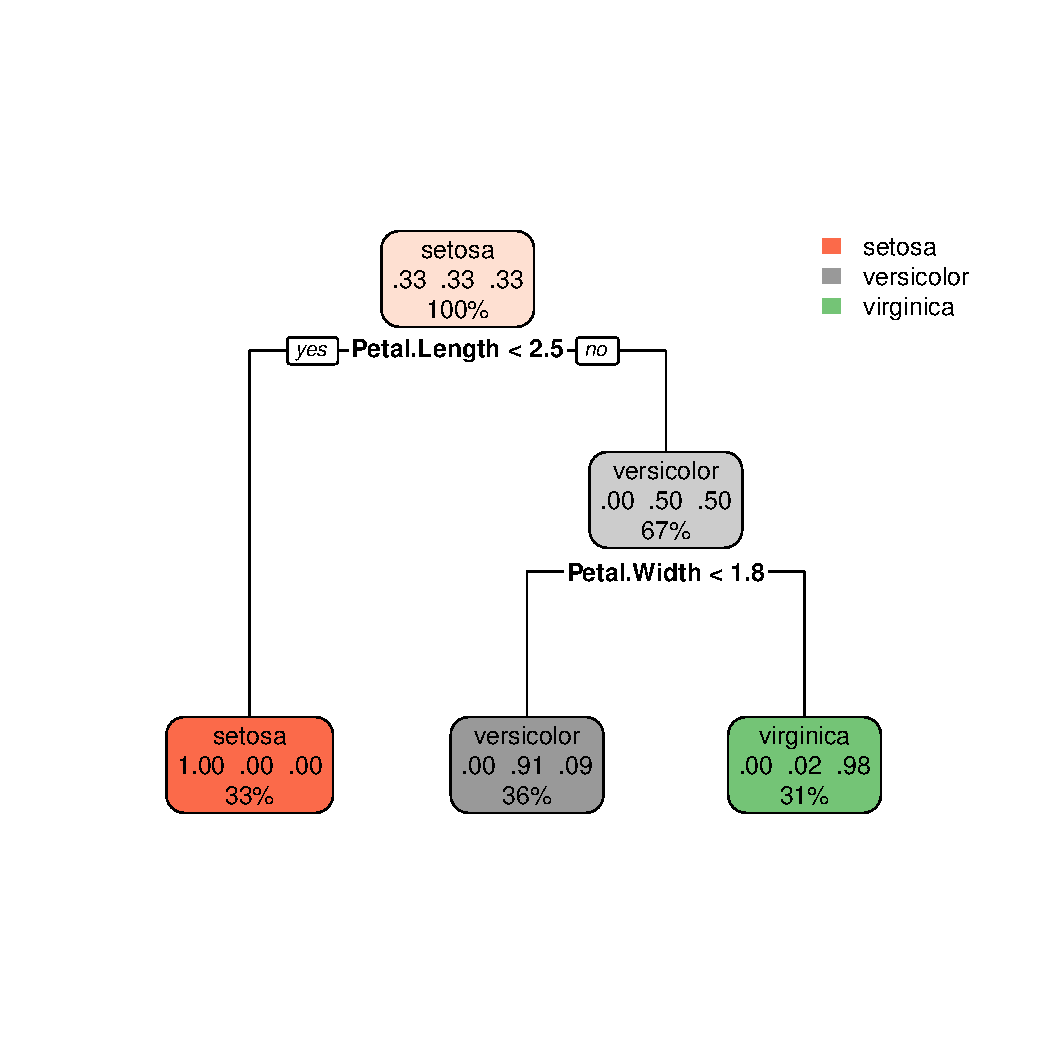
\includegraphics{./figures/tree_plot.pdf}
\caption{\label{fig:treePlot}Tree model structure.}
\end{figure}

\hypertarget{data-analysis}{%
\chapter{Data analysis}\label{data-analysis}}

\hypertarget{variable-filtering}{%
\section{Variable filtering}\label{variable-filtering}}

We performed variable filtering for variable importance and group variable importance. The procedure is as follows:

\begin{enumerate}
\def\labelenumi{\arabic{enumi}.}
\item
  Based on the initial variable importance or group variable importance where variables were ranked by the importance values, we first identified the most important set of variables or group variables by finding the largest importance gap between variables using an algorithm implementing an objective function.
\item
  From the remaining set of variables or group variables, we then selected the second most important set of variables or group variables with the largest gap observed in the remaining set.
\item
  We repeated Step 2 to find the third most important variable set and so on.
\item
  We trained multiple random forest models using the sets of variables we identified, where

  \begin{enumerate}
  \def\labelenumii{\alph{enumii}.}
  \tightlist
  \item
    the first random forest model was constructed using the \emph{most important} set of variables or group variables;
  \item
    the second random forest model was trained using the \emph{most important} and the \emph{second most important} variable sets;
  \item
    the third random forest model was built using the \emph{most important}, the \emph{second most important}, and the \emph{third most important} variables sets, and so on.
  \end{enumerate}
\item
  For each model with filtered variables, we evaluated the model performance using Akaike information criterion (AIC) (\protect\hyperlink{ref-Yun:2022tn}{Yun et al. 2022}; \protect\hyperlink{ref-rastgou2020estimating}{Rastgou et al. 2020}). The criterion is as follows:
  \begin{equation}
  n \times log(err) + 2 \times num\_vars,
  \label{eq:aic}
  \end{equation}
  where n is the number of samples, err is classification error or mean squared error (MSE) for regression. The criterion \eqref{eq:aic} accounts for both model error and number of variables. If there is a large number of variables in the training data set, the criterion will give more penalties to the model.
\item
  We reported random forest models having the \emph{lowest AIC values} for the variable filtering analysis.
\end{enumerate}

\hypertarget{references}{%
\chapter*{References}\label{references}}
\addcontentsline{toc}{chapter}{References}

\hypertarget{refs}{}
\begin{CSLReferences}{1}{0}
\leavevmode\vadjust pre{\hypertarget{ref-rastgou2020estimating}{}}%
Rastgou, M, H Bayat, Muharram Mansoorizadeh, and Andrew S Gregory. 2020. {``Estimating the Soil Water Retention Curve: Comparison of Multiple Nonlinear Regression Approach and Random Forest Data Mining Technique.''} \emph{Computers and Electronics in Agriculture} 174: 105502.

\leavevmode\vadjust pre{\hypertarget{ref-Yun:2022tn}{}}%
Yun, Daeun, Daeho Kang, Jiyi Jang, Anne Therese Angeles, JongCheol Pyo, Junho Jeon, Sang-Soo Baek, and Kyung Hwa Cho. 2022. {``A Novel Method for Micropollutant Quantification Using Deep Learning and Multi-Objective Optimization.''} \emph{Water Res} 212 (April): 118080. \url{https://doi.org/10.1016/j.watres.2022.118080}.

\end{CSLReferences}

\end{document}
